\subsection{Some extreme cases about Tutte's theorem}
In our project we do not use 3-connected graph but graph whose interior faces are triangle. It is obvious that considering the king of graphs we used Tutte's theorem is verified because the fypothesis « All interior faces are tringle » is lighter than « 3-connected » hypothesis. So now we changed the hypothesis about the external polyhgon and the interior vertices in order to find out if the tutte's algorithm is always verify.  

\subsubsection{Tutte's theorem and concave polygon}
Changing the hypothesis of the Tutte's theorem above, we try to prove that 

\begin {figure}[H]
  \centering
  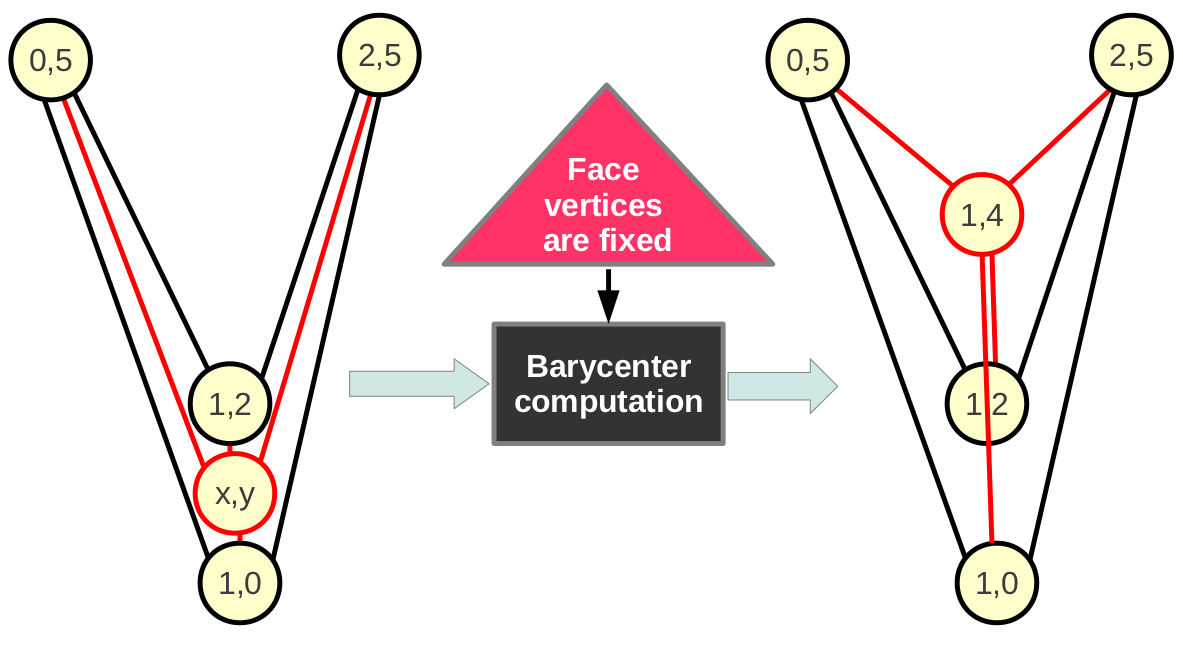
\includegraphics[scale=0.3]{img/tutte2.png}
  \caption{Tutte algorithm on concave polygon}
  \label{struct3}
\end {figure}

\subsubsection{Tutte's algorithm and convex polygon with some fixed vertices}


\begin {figure}[H]
  \centering
  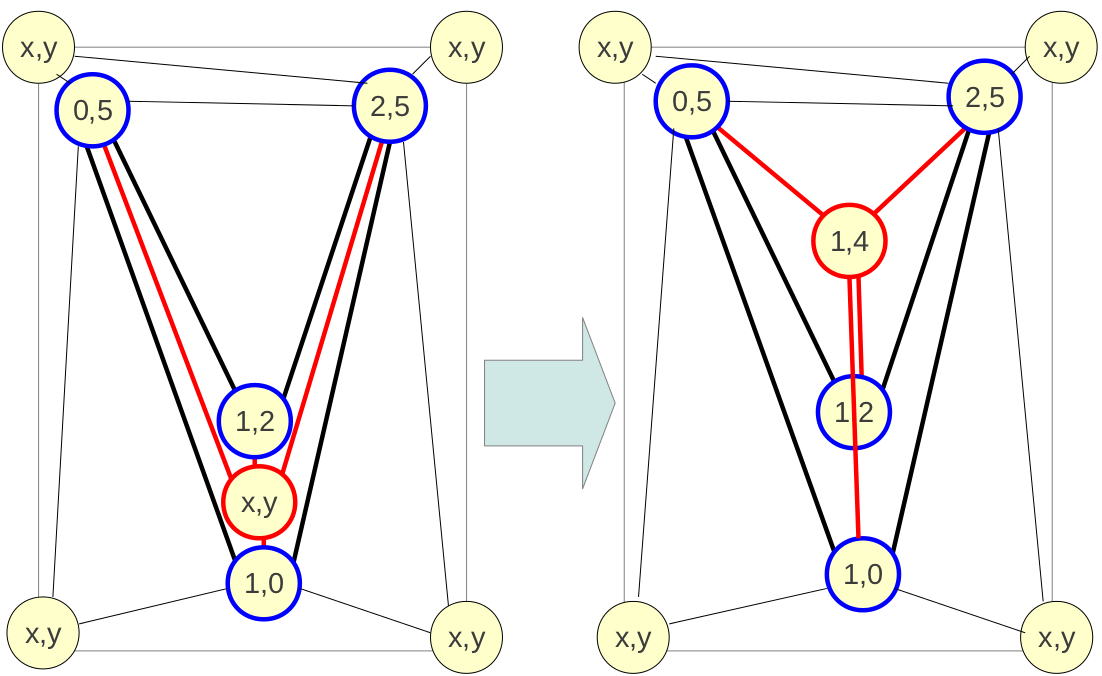
\includegraphics[scale=0.3]{img/tutte3.png}
  \caption{Tutte algorithme on convex polygon and fixes vertices}
  \label{struct3}
\end {figure}
